% This file was created with matplot2tikz v0.4.0.
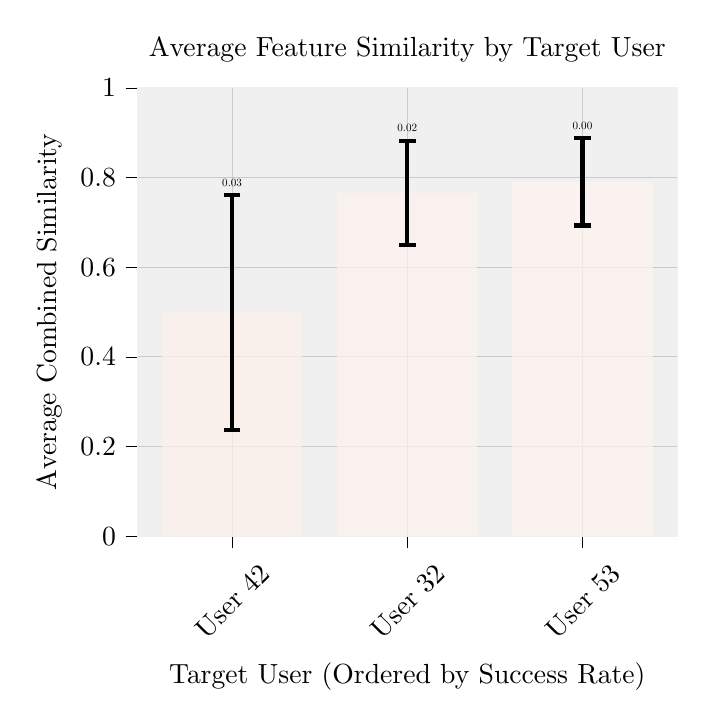
\begin{tikzpicture}

\definecolor{lightgray203}{RGB}{203,203,203}
\definecolor{linen254241234}{RGB}{254,241,234}
\definecolor{seashell254242236}{RGB}{254,242,236}
\definecolor{seashell254244239}{RGB}{254,244,239}
\definecolor{whitesmoke240}{RGB}{240,240,240}

\begin{axis}[
axis background/.style={fill=whitesmoke240},
axis line style={whitesmoke240},
tick align=outside,
tick pos=left,
title={Average Feature Similarity by Target User},
x grid style={lightgray203},
xlabel={Target User (Ordered by Success Rate)},
xmajorgrids,
xmin=-0.54, xmax=2.54,
xtick style={color=black},
xtick={0,1,2},
xticklabel style={rotate=45.0},
xticklabels={User 42,User 32,User 53},
y grid style={lightgray203},
ylabel={Average Combined Similarity},
ymajorgrids,
ymin=0, ymax=1,
ytick style={color=black}
]
\draw[draw=none,fill=linen254241234,fill opacity=0.7,very thin] (axis cs:-0.4,0) rectangle (axis cs:0.4,0.49914738469483);
\draw[draw=none,fill=seashell254242236,fill opacity=0.7,very thin] (axis cs:0.6,0) rectangle (axis cs:1.4,0.765398728900421);
\draw[draw=none,fill=seashell254244239,fill opacity=0.7,very thin] (axis cs:1.6,0) rectangle (axis cs:2.4,0.790358712227927);
\path [draw=black, ultra thick]
(axis cs:0,0.23733964929979)
--(axis cs:0,0.760955120089869);

\path [draw=black, ultra thick]
(axis cs:1,0.649118482684289)
--(axis cs:1,0.881678975116553);

\path [draw=black, ultra thick]
(axis cs:2,0.692903654911693)
--(axis cs:2,0.887813769544162);

\addplot [ultra thick, black, mark=-, mark size=3, mark options={solid}, only marks]
table {%
0 0.23733964929979
1 0.649118482684289
2 0.692903654911693
};
\addplot [ultra thick, black, mark=-, mark size=3, mark options={solid}, only marks]
table {%
0 0.760955120089869
1 0.881678975116553
2 0.887813769544162
};
\draw (axis cs:0,0.780955120089869) node[
  scale=0.4,
  anchor=base,
  text=black,
  rotate=0.0
]{0.03};
\draw (axis cs:1,0.901678975116553) node[
  scale=0.4,
  anchor=base,
  text=black,
  rotate=0.0
]{0.02};
\draw (axis cs:2,0.907813769544162) node[
  scale=0.4,
  anchor=base,
  text=black,
  rotate=0.0
]{0.00};
\end{axis}

\end{tikzpicture}
